\documentclass[aspectratio=1610]{beamer}

\usepackage{makecell}
\usepackage{etoolbox}
\usepackage{biblatex}

\usepackage{tikz} % for graph

\usepackage{bbding}
\usepackage{layouts}
\usepackage{hyperref} % hyper text

\usepackage{booktabs} % To thicken table lines

\usepackage[normalem]{ulem} % for striking words

%margins
\newenvironment{changemargin}[2]{%
\begin{list}{}{%
\setlength{\topsep}{0pt}%
\setlength{\leftmargin}{#1}%
\setlength{\rightmargin}{#2}%
\setlength{\listparindent}{\parindent}%
\setlength{\itemindent}{\parindent}%
\setlength{\parsep}{\parskip}%
}%
\item[]}{\end{list}}

% code formating
\usepackage{xcolor}
\usepackage{listings} 
\lstset{basicstyle=\ttfamily,
  showstringspaces=false,
  commentstyle=\color{red},
  keywordstyle=\color{blue}
}
\definecolor{codegreen}{rgb}{0,0.6,0}
\definecolor{codegray}{rgb}{0.5,0.5,0.5}
\definecolor{codepurple}{rgb}{0.58,0,0.82}
\definecolor{backcolour}{rgb}{0.95,0.95,0.92}

\lstdefinestyle{mystyle}{
  backgroundcolor=\color{backcolour},   
  commentstyle=\color{codegreen},
  keywordstyle=\color{magenta},
  numberstyle=\tiny\color{codegray},
  stringstyle=\color{codepurple},
  basicstyle=\ttfamily\footnotesize,
  breakatwhitespace=false,         
  breaklines=true,                 
  captionpos=b,                    
  keepspaces=true,                 
  numbers=left,                    
  numbersep=5pt,                  
  showspaces=false,                
  showstringspaces=false,
  showtabs=false,                  
  tabsize=2
}



% ADD '-pdflua' as argument of latexmk
% Ref https://mirror.ibcp.fr/pub/CTAN/macros/luatex/latex/emoji/emoji-doc.pdf
\usepackage{emoji}
% For linux :https://github.com/samuelngs/apple-emoji-linux
\setemojifont{Apple Color Emoji}

\usepackage[sfdefault]{FiraSans}
\usetheme{metropolis}           % Use metropolis theme
\usetikzlibrary{positioning,shapes,arrows,calc,fit,backgrounds,shapes.multipart}

\tikzset{box/.style={draw, rectangle, rounded corners, thick, node distance=7em, text width=6em, text centered, minimum height=3.5em}}
\tikzset{line/.style={draw, thick, -latex'}}
\tikzset{every node/.style={font=\scriptsize}}

%Graphics and Videos
% https://tex.stackexchange.com/questions/89088/how-to-embed-video-and-animation-in-latex-and-latex-beamer-step-by-step
\usepackage{graphicx} %The mode "LaTeX => PDF" allows the following formats: .jpg  .png  .pdf  .mps
\usepackage{animate}


%\usepackage[utf8]{inputenc}
%\usetheme{Antibes}
\usefonttheme{professionalfonts}

\setbeamertemplate{itemize items}[circle]

%\bibliography{presentation}

\newcommand\blfootnote[1]{%
  \begingroup
  \renewcommand\thefootnote{}\footnote{{\tiny #1}}%
  \addtocounter{footnote}{-1}%
  \endgroup
}


%Page de titre:
\title[\emoji{dna} Analyse Exome ??? ]{\emoji{dna} Analyse Exomes ??? }


\author{Dr. Thomas Steimlé}
\institute[OH]{
  Laboratoire d'oncohématologie de l'hôpital Necker \\
  \vfill
  \begin{figure}[!b]
    \centering
    
\includegraphics[height=1cm]{Images/1200aphp.pdf}\hspace*{5.5cm}~
    
\includegraphics[height=1.5cm]{Images/necker.pdf}
  \end{figure}
}
\date{Août 2021}

%\titlegraphic{\hfill\includegraphics[height=1.5cm]{Images/1200aphp.svg.png}}
%\logo{\includegraphics[width=3cm]{Images/1200aphp.svg.png}}
\begin{document}

\begin{frame}
\maketitle
\thispagestyle{empty}

\end{frame}
%\frame{\titlepage}
%\logo{}

\begin{frame}
  \frametitle{\emoji{dart} Objectif}
  \begin{itemize}
    \item Dans les ??? , identifier des gènes d'intérêts à inclure dans un panel NGS ciblé.
  \end{itemize}
\end{frame}

\begin{frame}
  \frametitle{\emoji{test-tube} Matériels }
  \begin{center}
  \textbf{N = 11} couples normal/tumoral (FFPE). \\
  Les prélèvement tumoraux ont été qualifiés en anapath (???) et en CG ().
  \begin{footnotesize}
  \begin{table}
    \begin{tabular}[tl]{lcc}
      \toprule
        \textbf{Case} & \textbf{\emoji{microscope} Infiltration} & \textbf{Commentaire} \\
      \midrule
        ???02	& 60\% & \\
        ???05	& 80\% & \\
        \sout{???11}	& 70\% & \emoji{cross-mark} échantillon normal prélevé après allo-HSCT \\
        ???23	& 90\% & \\
        ???24	& 80\% & \\
        ???51	& 60\% & \\
        ???53	& 60\% & \\
        ???55	& 90\% & \\
        ???65	& 70\% & \\
        \sout{???81}	& 60\% & \emoji{cross-mark} échantillon de qualité insuffisante\\
        ???89	& 60\% & \\
        ???90	& 70\% & \\
        ???94	& 50\% & \\ 
      \bottomrule
    \end{tabular}
  \end{table}
  \end{footnotesize}
  \end{center}
\end{frame}

\begin{frame}
  \frametitle{\emoji{straight-ruler} Méthodes}
  \begin{itemize}
    \item[] \emoji{dna} Séquençage selon la méthode \textit{Agilent SureSelect Human All Exon V7 panel} sur automates \textit{Illumina Next/NovaSeq}.
    \vskip 0.2in
    \item[] \emoji{floppy-disk} Analyse bioinformatique réalisée à partir des BAM fournis par Imagine.
    \vskip 0.1in
    Callers : 
    \vskip 0.05in
    \begin{itemize}
      \item \textbf{mutect2} (GATK v4.2)
      \item \textbf{strelka} (Illumina v2.9.10)
      \item \textbf{lancet} (NY Genome Center v1.1.0)
    \end{itemize}
    \vskip 0.05in
    \item[] En suivant les modes opératoires fournis (cf. diapos supplémentaires).
  \end{itemize}
\end{frame}


\section{\emoji{chart-increasing} Résultats}

\begin{frame}
  \frametitle{\emoji{warning} Problèmes sur les couples N/P 11 et 81}
  \begin{center}
    \begin{figure}
        \centering
      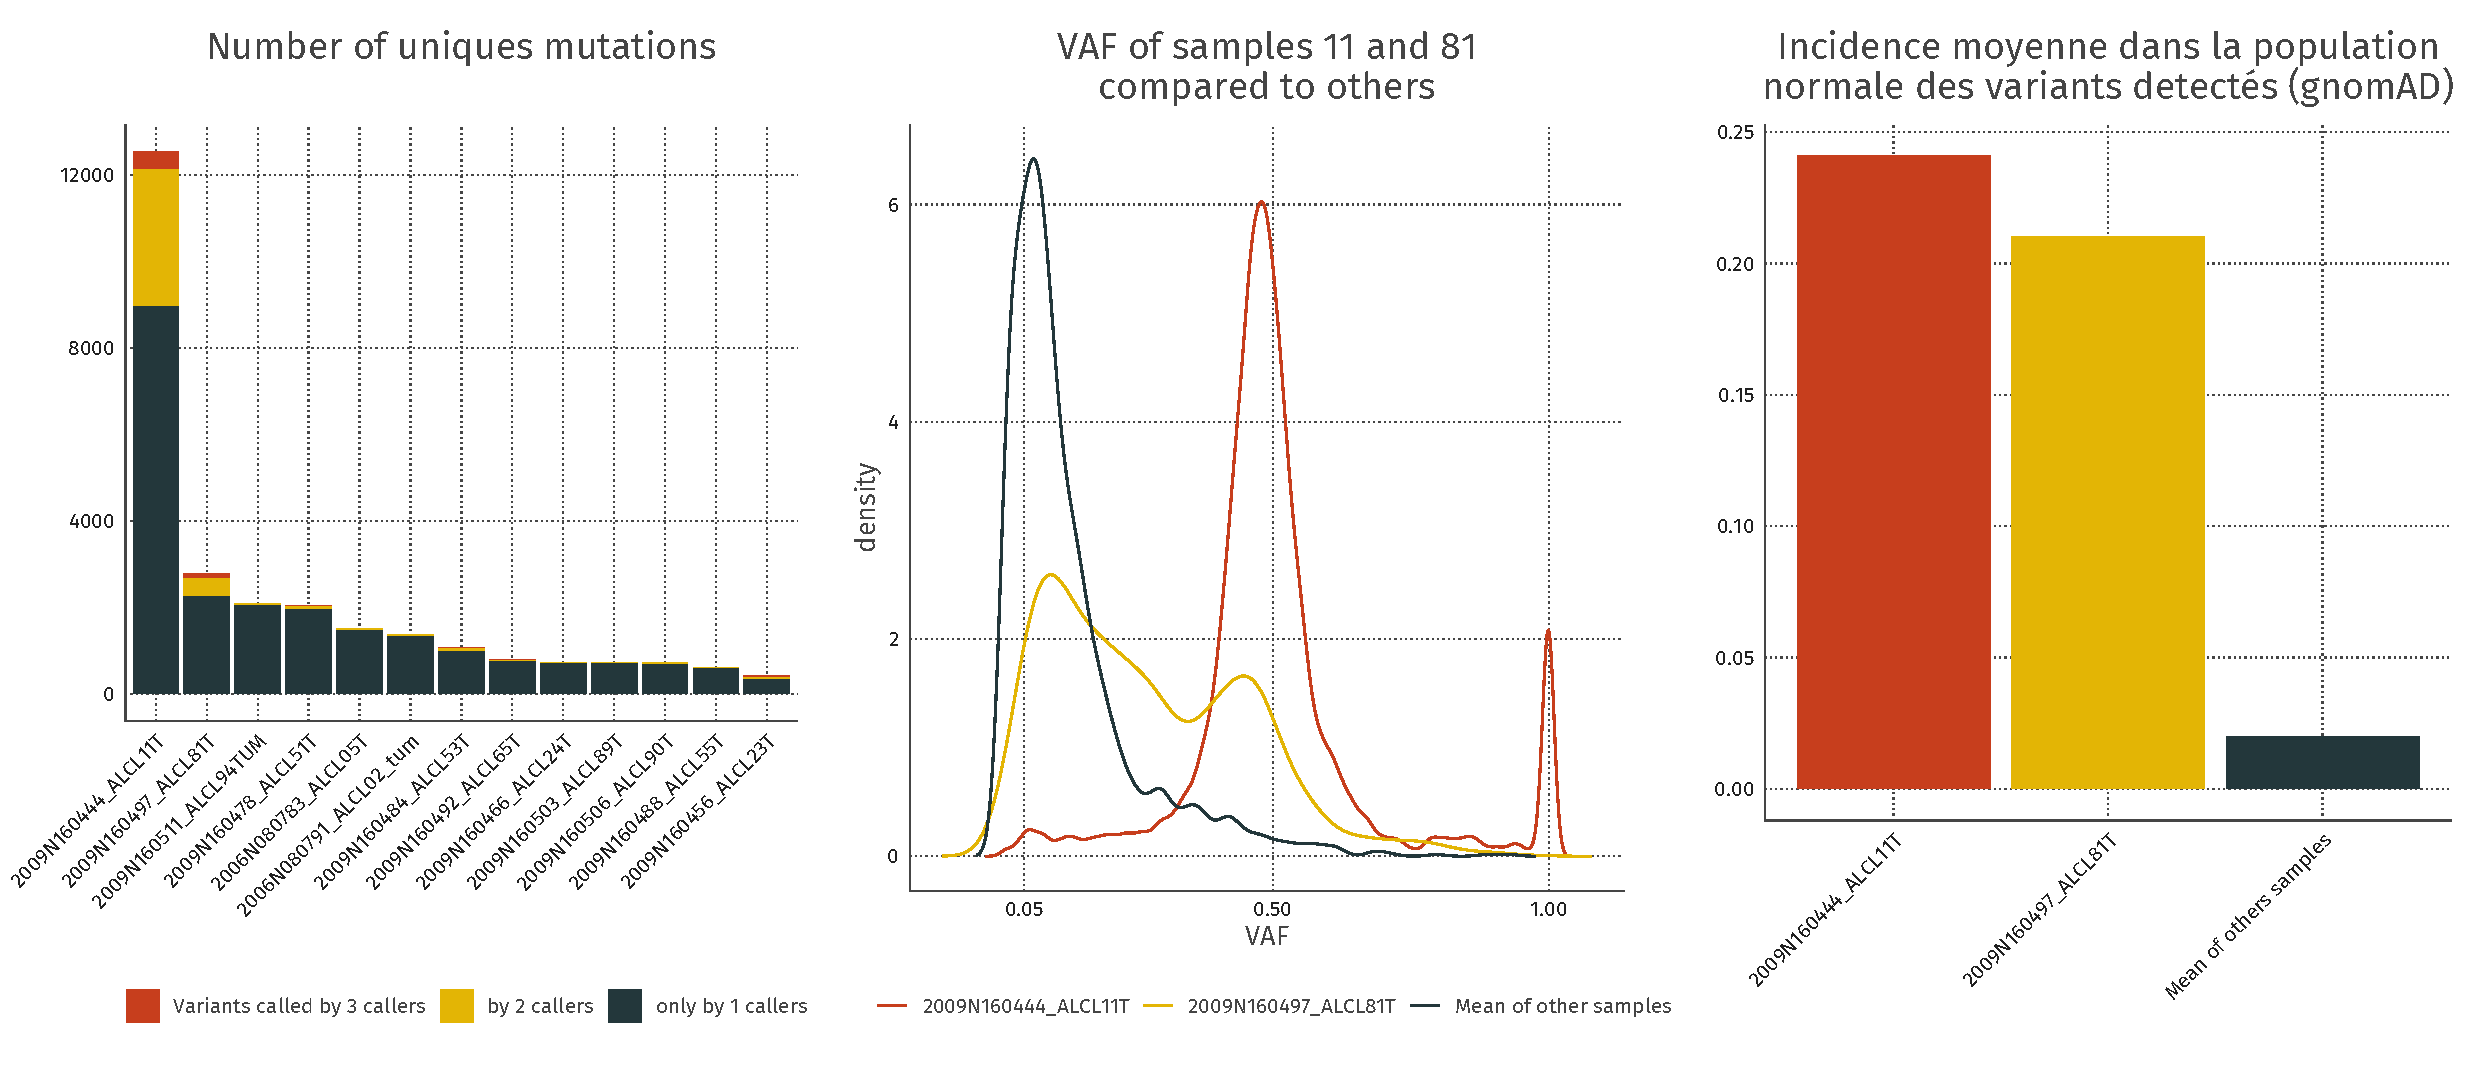
\includegraphics[width=\textwidth]{Images/Qual.pdf}
    \end{figure}
  \end{center}
  \begin{itemize}
    \item Détection d'un nombre trop important de SNP dans les échantillons 11 et 81.
    \item En raison pour le 11 d'un "normal" prélevé après allo-HSCT.
  \end{itemize}
  \textbf{
    \emoji{right-arrow}  Couples 11 et 81 non inclus dans l'analyse \emoji{heavy-exclamation-mark}
  }
\end{frame}

\begin{frame}
  \frametitle{\emoji{put-litter-in-its-place} Filtrage des variants}
  \begin{center}
    \begin{figure}
      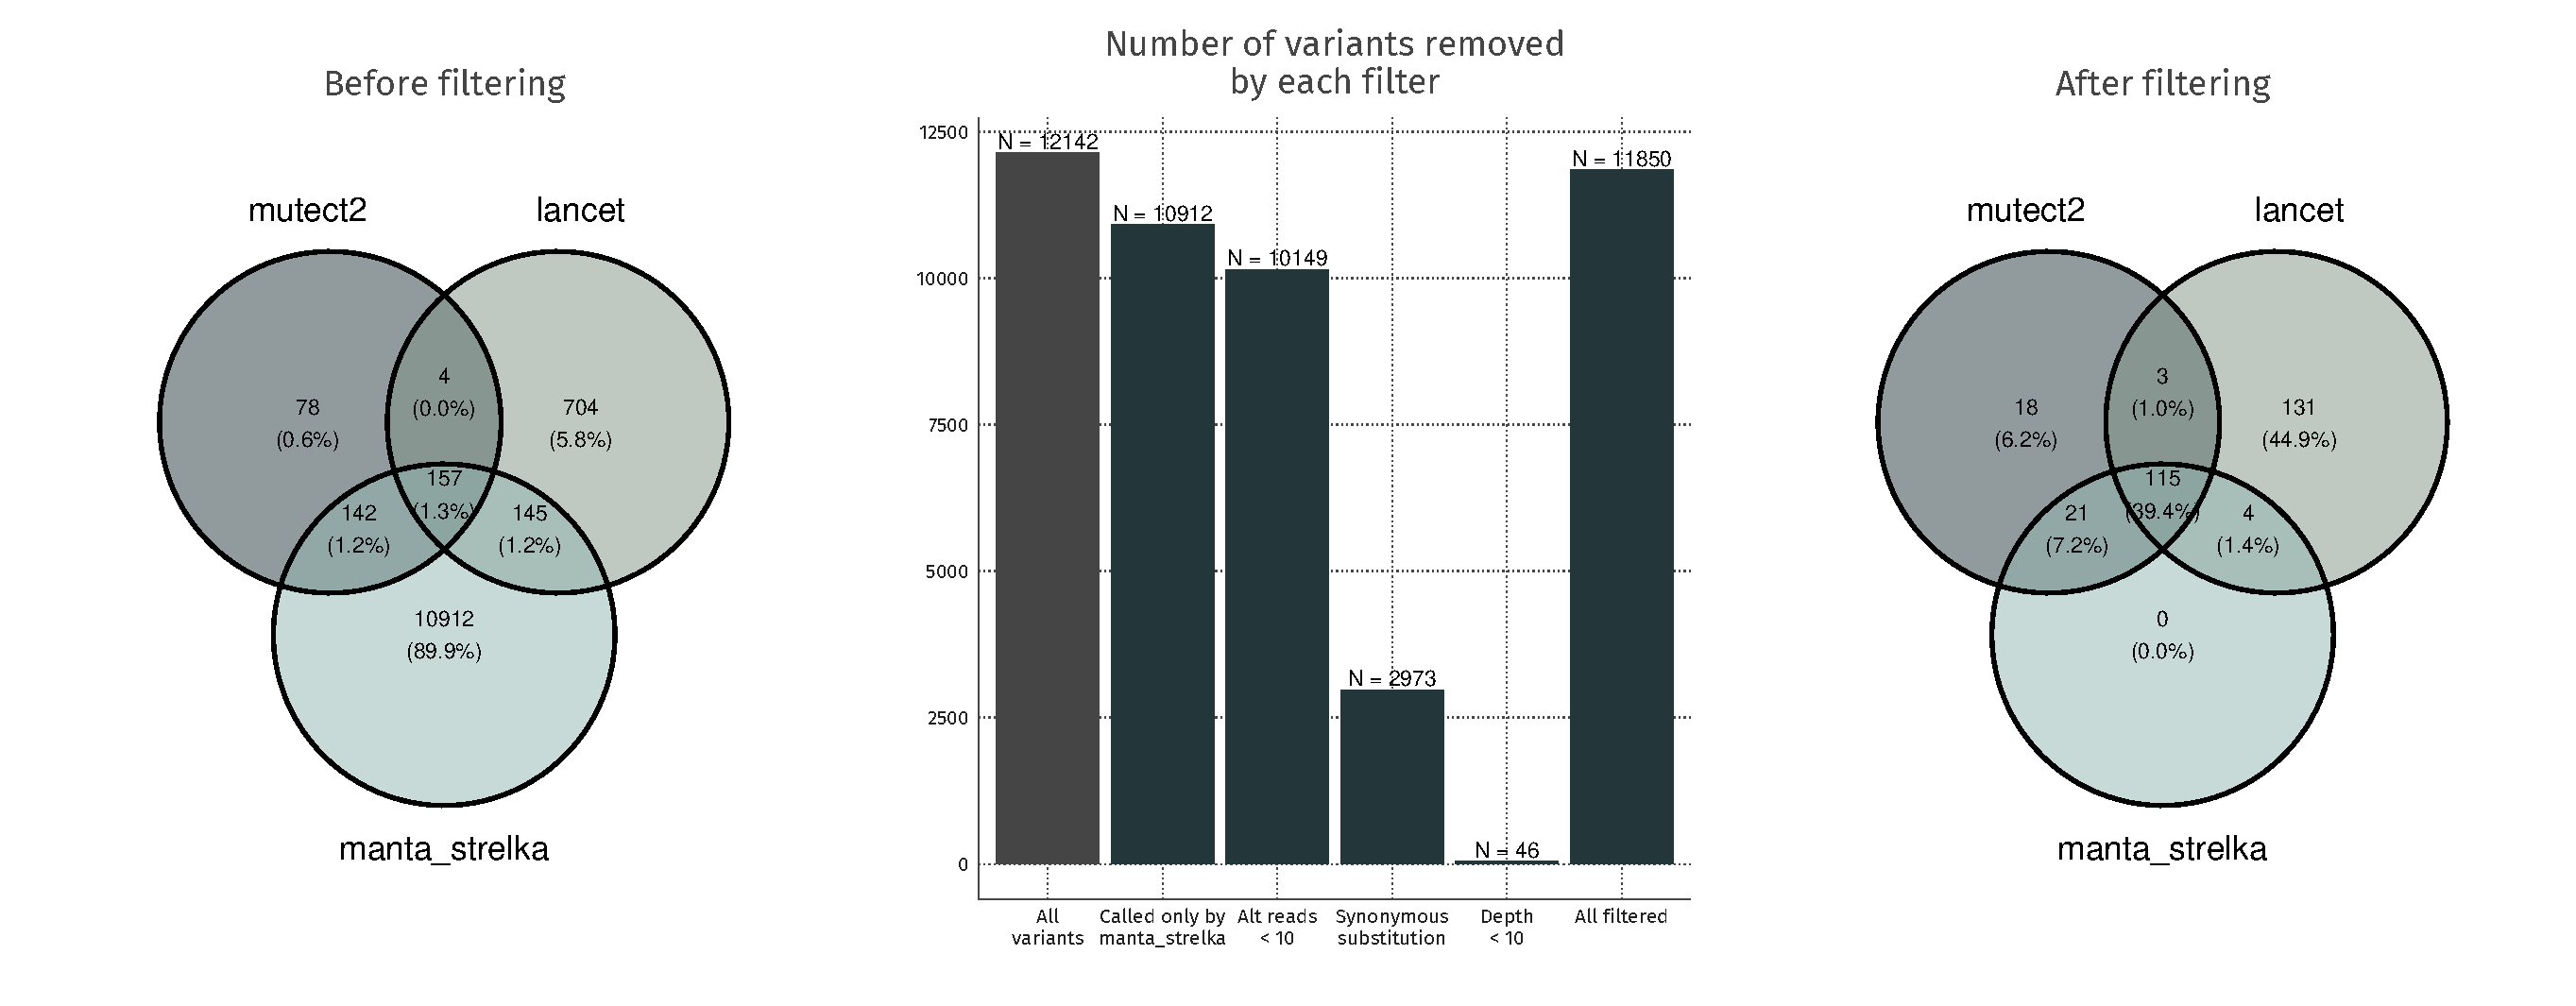
\includegraphics[width=\textwidth]{Images/Filtering_A.pdf}
    \end{figure}
  \end{center}
  \begin{itemize}
    \item Le caller manta\_strelka est peu spécifique (89\% des mutations) on s'en servera uniquement pour confirmation.
  \end{itemize}
  \textbf{
    \emoji{right-arrow} 292 variants sélectionnés (2,4\%)
  }
\end{frame}

\begin{frame}
  \frametitle{\emoji{put-litter-in-its-place} Filtrage des variants}
  \begin{center}
    \begin{figure}
      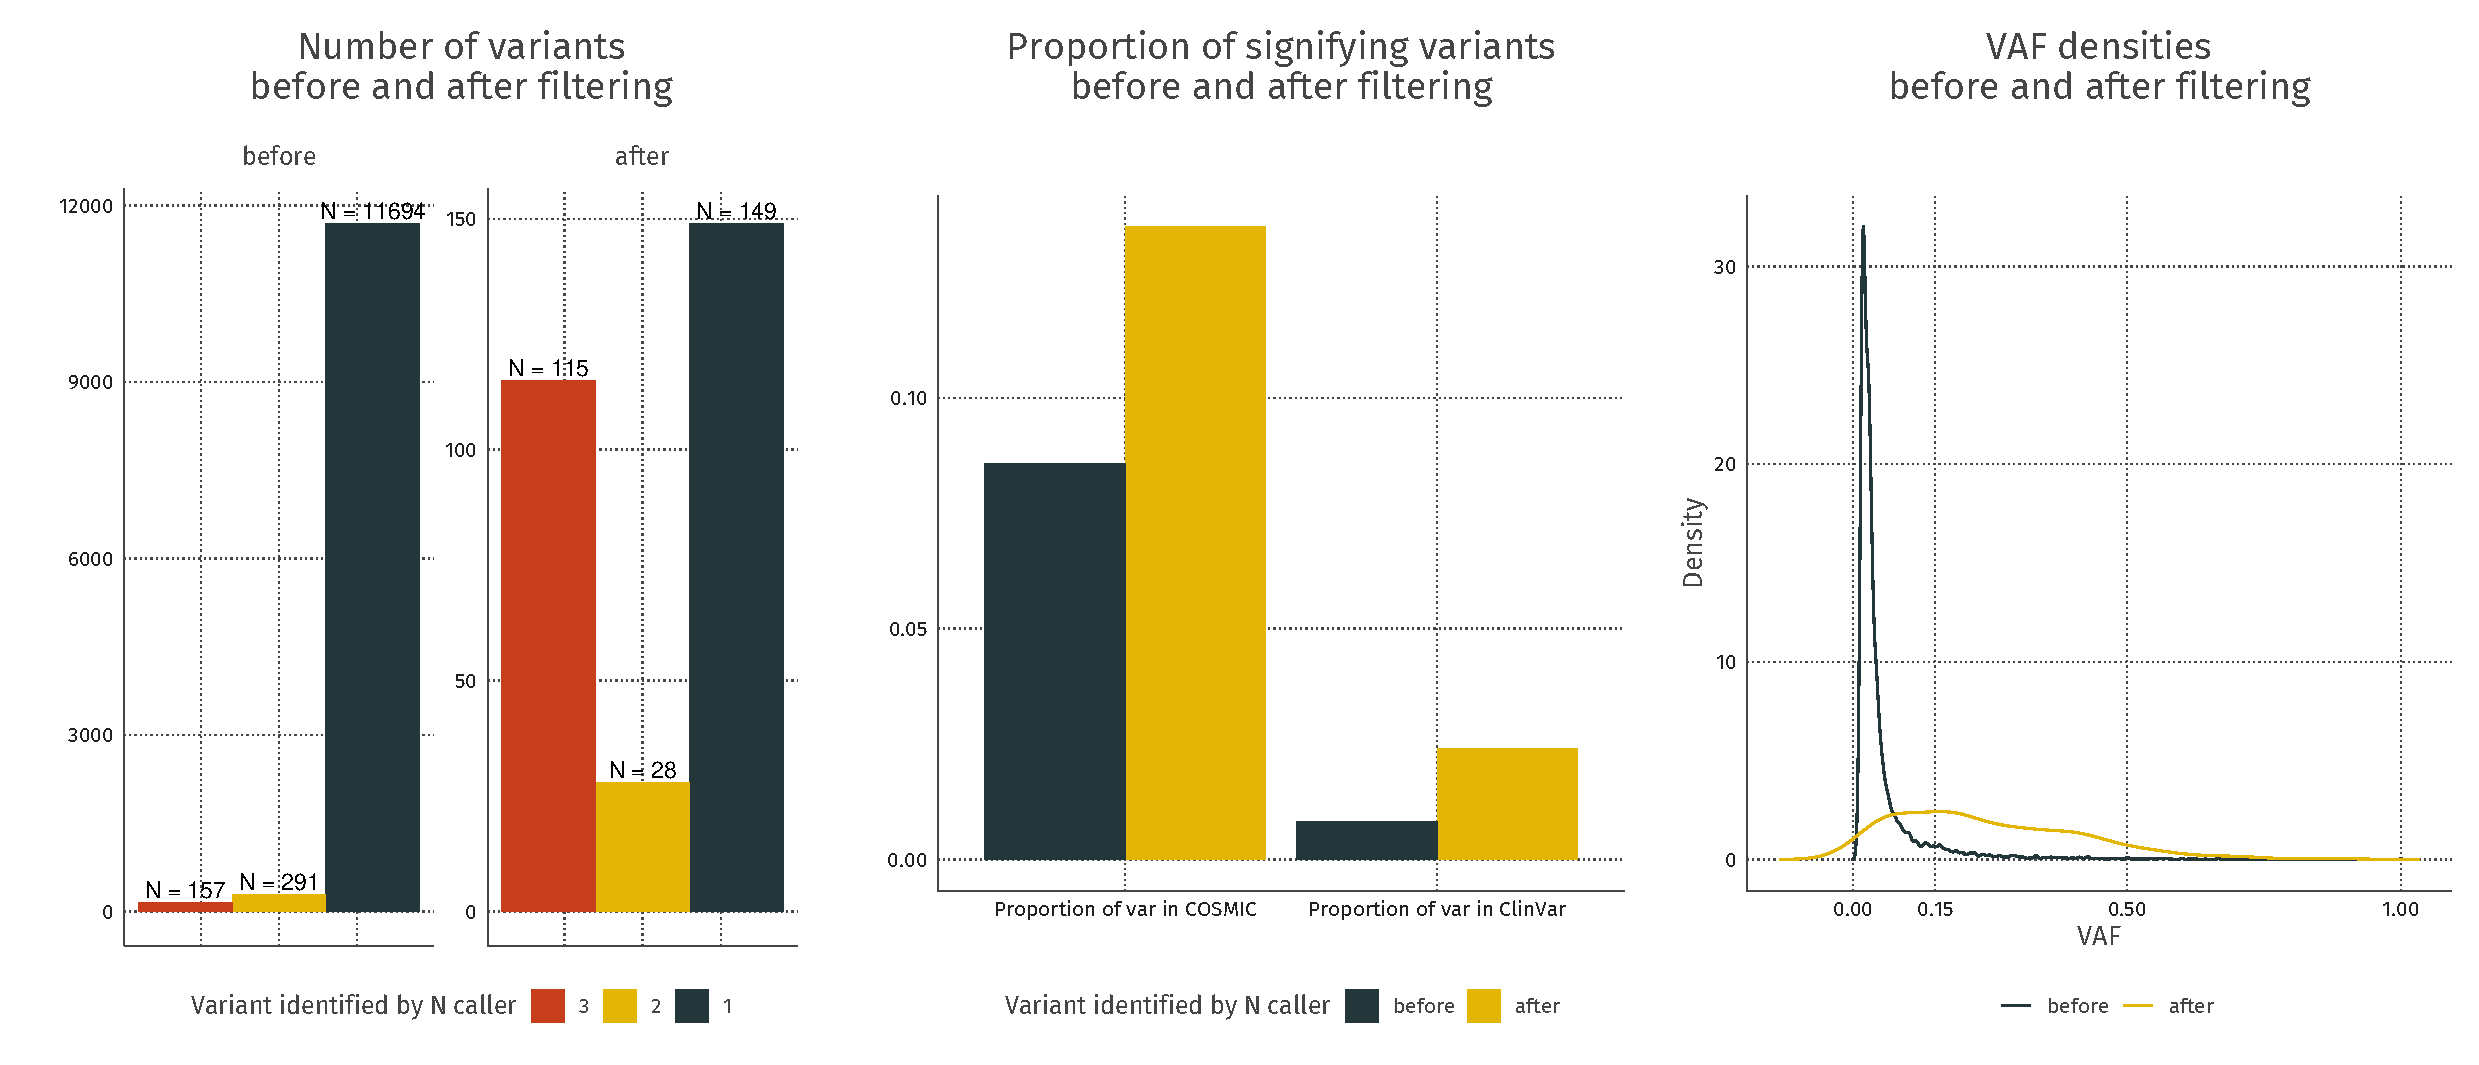
\includegraphics[width=\textwidth]{Images/Filtering_B.pdf}
    \end{figure}
  \end{center}
  Les variants sélectionnés sont plus fréquemment appelés par \textbf{plusieurs callers}. Présentent une proportion plus importante de \textbf{variants significatifs} et sont de \textbf{VAF compatible avec l'infiltration}.
\end{frame}

\begin{frame}
  \frametitle{\emoji{arrows-counterclockwise} Gènes mutés plusieurs fois dans la cohorte (N = 11)}  
  \begin{center}
    UNPUBLISHED DATA
  \end{center}
\end{frame}

\begin{frame}
  \frametitle{\emoji{mag-right} }
  \begin{center}
    UNPUBLISHED DATA
  \end{center}  
\end{frame}

\begin{frame}
  \frametitle{\emoji{card-index-dividers} Mutations clonales significatives mais non récurrentes dans la cohorte}
  \begin{center}
    UNPUBLISHED DATA
  \end{center}
\end{frame}

\begin{frame}
  \frametitle{\emoji{card-index-dividers} Mutations clonales significatives mais non récurrentes dans la cohorte}
  \begin{center}
    UNPUBLISHED DATA
  \end{center}
\end{frame}

\begin{frame}[standout]
  Supplementary
\end{frame}

\begin{frame}
  \frametitle{\emoji{floppy-disk} Méthodes > Calling > Lancet}
  Source code : \url{https://github.com/nygenome/lancet}
  \vskip 0.2in
  \lstinputlisting[language=bash, caption={lancet -- bash version}, style=mystyle]{Codes/lancet.txt}
\end{frame}

\begin{frame}
  \frametitle{\emoji{floppy-disk} Méthodes > Calling > Manta puis Strelka}
  \begin{footnotesize}
    Manta : \url{https://github.com/Illumina/manta}
    \lstinputlisting[language=bash, caption={manta -- bash version}, style=mystyle]{Codes/manta.txt}
    Strelka : \url{https://github.com/Illumina/strelka}
    \lstinputlisting[language=bash, caption={strelka -- bash version}, style=mystyle]{Codes/strelka.txt}
  \end{footnotesize}
\end{frame}

\begin{frame}
  \frametitle{\emoji{floppy-disk} Méthodes > Calling > Mutect2}
  Les étapes ont été reproduites à partir de : \footnotesize \url{https://gatk.broadinstitute.org/hc/en-us/articles/360035531132}
  \lstinputlisting[language=bash, caption={Mutect2 -- seule étape adaptée -- bash version}, style=mystyle]{Codes/mutect2.txt}
\end{frame}



\end{document}
